
\documentclass[11pt]{article}
\usepackage{amsmath,amssymb}
\usepackage{graphicx}
\usepackage[margin=0.75in]{geometry}
\usepackage{bm}
\usepackage{color}
\usepackage[usenames,dvipsnames]{xcolor}
\usepackage{enumerate}
\usepackage{courier}
\usepackage{float}
\usepackage{verbatim}

\setlength\parindent{0pt}
\newcommand{\pr}{P} % Generic probability
\newcommand{\var}{\textrm{Var}}
\newcommand{\cov}{\textrm{Cov}}


\title{STAT 240 Homework 4}
\author{Rebecca Barter, Andrew Do, and Kellie Ottoboni}
\date{May 1, 2015} % delete this line to display the current date

%%% BEGIN DOCUMENT
\begin{document}

\maketitle


\section*{Problem (1)}
We completed the code in file \texttt{hw4\_functions.R}.  For the dataset 
$$X: -1.0, 1.7, -2.0, 0.6, 0.9, 3.5, \qquad Y : 1.9, -0.3, 2.8, -0.7, 1.6, -2.4$$

we obtained the following p-values setting $\texttt{L}$ to 1,000,000.
\begin{table}[htdp]
\begin{center}
\begin{tabular}{|c|c|c|c|c|}
\hline
 & z Statistic & Wilcoxon Rank Sum & Paired z & Signed Rank  \\ \hline
Normal Approximation & 0.4505772 & 0.5319069 & 0.4625569 & 0.5   \\
Permutation & 0.454514 & 0.531657 & 0.455443 & 0.499427  \\ \hline
\end{tabular}
\end{center}
\label{default}
\end{table}%
 The exact p-value for the sign test was $0.65625$.  Next, we use the dataset 
$$X: 0.5, 2.4, -4.1, 5.9, 3.7, 3.6, \qquad Y : 2.7, 0.8, 1.6, 5.7, 4.3, 0.3$$

We obtained the following p-values setting $\texttt{L}$ to 1,000,000.
\begin{table}[htdp]
\begin{center}
\begin{tabular}{|c|c|c|c|c|}
\hline
 & z Statistic & Wilcoxon Rank Sum & Paired z & Signed Rank  \\ \hline
Normal Approximation & 0.6393479 & 0.5319069 & 0.6826982 & 0.6625066   \\
Permutation & 0.626417 &  0.531804 & 0.626229 & 0.655774  \\ \hline
\end{tabular}
\end{center}
\label{default}
\end{table}%

The p-value for the sign test was $ 0.65625$.

\newpage
\section*{Problem (2)}
We estimated the power for each of the five tests from part (1) by generating 100,000 datasets (where $X$ and $Y$ each have sample size 50) according to the specified distribution, and identifying the fraction of null hypotheses rejected at the 0.05 significance level using the normal approximation (except for the sign test). The results are presented in Figure \ref{fig:part2} and Table \ref{tab:part2}.


\begin{figure}[H]
\centering
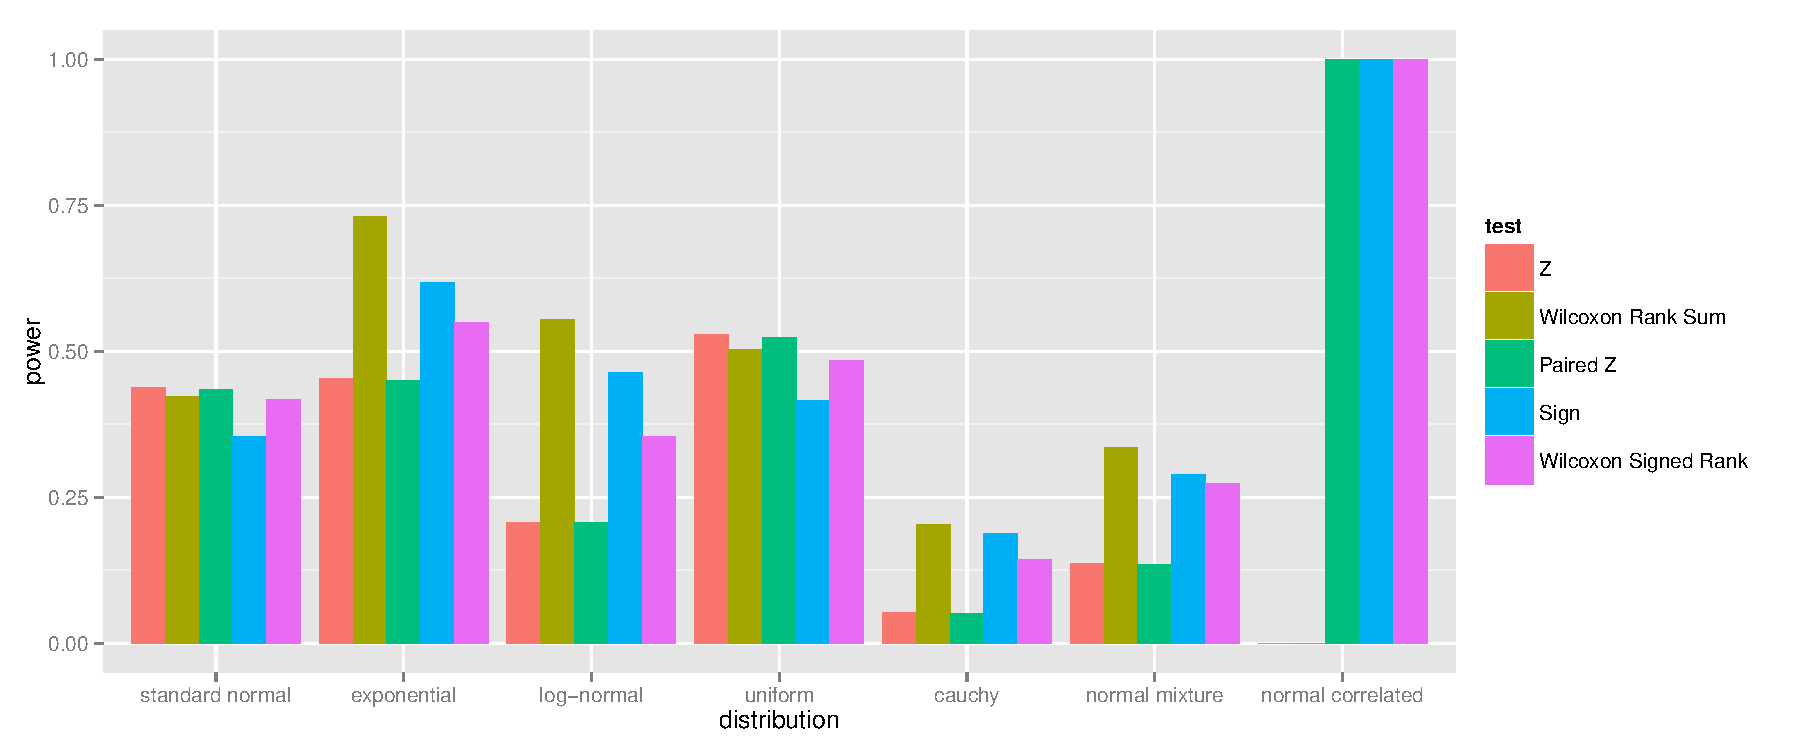
\includegraphics[scale = 0.8]{part2.pdf}
\caption{The power of each test where $Y$ has each of the stated distributions and $X$ has the same distribution as $Y$, but is shifted up by 0.3.}
\label{fig:part2}
\end{figure}


\begin{table}[ht]
\centering
\begin{tabular}{lrrrrrrr}
  \hline
 test & std normal & exp & lognormal & uniform & cauchy & normal mix. & normal corr. \\ 
  \hline
Z & 0.44 & 0.53 & 0.00 & 0.21 & 0.14 & 0.45 & 0.05 \\ 
 Wilcoxon Rank Sum & 0.01 & 0.00 & 0.00 & 0.00 & 0.00 & 0.00 & 0.00 \\ 
 Paired Z & 0.45 & 0.05 & 0.43 & 0.52 & 1.00 & 0.21 & 0.13 \\ 
  Sign & 0.00 & 0.00 & 0.01 & 0.00 & 0.00 & 0.00 & 0.00 \\ 
 Wilcoxon Signed Rank & 0.35 & 0.27 & 0.55 & 0.14 & 0.42 & 0.48 & 1.00 \\ 
   \hline
\end{tabular}
\caption{The power of each test where $Y$ has each of the stated distributions and $X$ has the same distribution as $Y$, but is shifted up by 0.3.}
\label{tab:part2}
\end{table}

\noindent We see that in each of these scenarios, the $Z$-test has highest power (approximately 0.5) when our data comes from an exponential distribution, the standard normal distribution or a normal mixture distribution. The Wilcoxon rank-sum test and the sign test both seem to have very low power for all distributions considered, the paired $Z$-test has extremely high power when the data comes from a Cauchy distribution, and  has power of approximately 0.5 when the data comes from a standard normal, lognormal or uniform distribution. The Wilcoxon signed rank test has extremely high power when the data comes from a normal distribution but $X$ and $Y$ are correlated, and has power of approximately 0.5 for the lognormal and normal mixture distributions.\\
Thus, overall, it appears as though the Wilcoxon signed rank test is more powerful than the paired $Z$ test for the exponential distribution, lognormal distribution, normal mixture distribution and normal distribution where $X$ and $Y$ are correlated. However, paired $Z$ test is more powerful for the standard normal, uniform and Cauchy distributions.\\
On the other hand, the $Z$ test is more powerful than the Wilcoxon Rank Sum test in all cases except when the data comes from a lognormal distribution.


\end{document}